\documentclass[addpoints]{exam}
\usepackage{url}
\usepackage{amsmath,amsthm,enumitem, amssymb} 
\usepackage{mathtools}
\usepackage{amssymb}
\usepackage{graphicx}
\usepackage{qtree}
\usepackage[nodayofweek,level]{datetime}
\usepackage{color}
\usepackage{csquotes}
\usepackage{pgf, tikz}
\usetikzlibrary{arrows, automata}
\usepackage{algorithm,algpseudocode}
\usepackage{graphicx}
\usepackage{pgfplots}
\usetikzlibrary{patterns}
\usetikzlibrary{positioning}
\usetikzlibrary{calc,arrows.meta,positioning}

\tikzset{
    every node/.style={font=\sffamily\small},
    main node/.style={thick,circle,draw,font=\sffamily\Large}
}
\newtheorem*{claim}{Claim}
\definecolor{qcolor}{rgb}{0, 0, 0.3}
\definecolor{acolor}{rgb}{0, 0, 0}
%\input myfonts
\qformat{Question \thequestion: \thequestiontitle\dotfill \textbf{[\totalpoints]}}
\pointname{}
\bonuspointname{}
\pointformat{[\bfseries\thepoints]}

\lhead{Gopal Menon (u0772360)}
\chead{\bf{HW5}}
\rhead{CS 6150 \today}
\headrule

\makeatletter
\newcommand{\pgfplotsdrawaxis}{\pgfplots@draw@axis}
\makeatother
\pgfplotsset{only axis on top/.style={axis on top=false, after end axis/.code={
             \pgfplotsset{axis line style=opaque, ticklabel style=opaque, tick style=opaque,
                          grid=none}\pgfplotsdrawaxis}}}

\newcommand{\drawge}{-- (rel axis cs:1,0) -- (rel axis cs:1,1) -- (rel axis cs:0,1) \closedcycle}
\newcommand{\drawle}{-- (rel axis cs:1,1) -- (rel axis cs:1,0) -- (rel axis cs:0,0) \closedcycle}

\begin{document}

\section*{Collaborators}

Ben Nelson, Corbin Baldwin and I collaborated for this assignment.

\begin{questions}

\titledquestion{Basics of linear programming}
Consider the feasible set of the following set of inequalities in two variables $x, y$:
\begin{align*}
x + y &\ge 1, \\
x + 2y &\le 4, \\
y &\le 2.
\end{align*}
\begin{parts}
\part[3] Draw the feasible region on the plane (you may also draw on paper, roughly to scale, and attach a scanned image).
\part[2] What is the maximum value of $x+4y$ subject to $(x, y)$ being in the feasible region?
\part[2] Answer the same for $x+y$.
\part[2] Find a point $(x,y)$ that is the intersection of two of the lines defining the equations above, but is not a corner point of the feasible region.
\end{parts}

\begin{parts}

\part The feasible region is shown below in cyan. It is unbounded on the bottom-right.
  
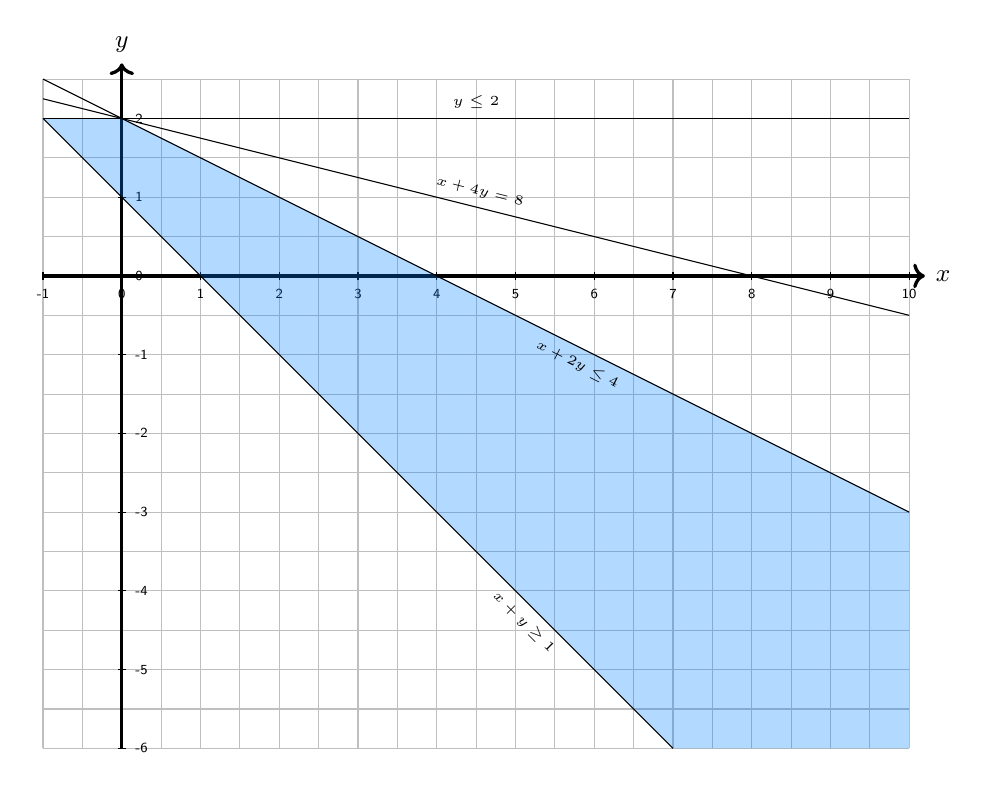
\begin{tikzpicture}

    \draw[gray!50, thin, step=0.5] (-1,-6) grid (10,2.5);
    \draw[very thick,->] (-1,0) -- (10.2,0) node[right] {$x$};
    \draw[very thick,->] (0,-6) -- (0,2.7) node[above] {$y$};

    \foreach \x in {-1,...,10} \draw (\x,0.05) -- (\x,-0.05) node[below] {\tiny\x};
    \foreach \y in {-6,...,2.5} \draw (-0.05,\y) -- (0.05,\y) node[right] {\tiny\y};

    \fill[blue!50!cyan,opacity=0.3] (-1,2) -- (0,2) -- (10,-3) -- (10,-6) -- (7,-6) -- cycle;

    \draw (-1,2)  -- (3.5,-2.5) --  node[below,sloped] {\tiny$x+y\geq1 $} (7,-6);
    \draw (-1, 2.5) -- (3,0.5) --  node[below left,sloped] {\tiny$x+2y\leq4$} (10,-3);
    \draw (-1,2) -- node[above,sloped] {\tiny$y\leq2$} (10,2);
    \draw (-1,2.25) -- node[above,sloped] {\tiny$x+4y=8$} (10,-1/2);

\end{tikzpicture}

\part The maximum value of $x+4y$ subject to $(x, y)$ being in the feasible region will be at the corner $(0, 2)$ as shown above.

\part We can try and find the maximum value of $x+y$ subject to $(x, y)$ being in the feasible region, by moving the line $x+y=1$ (the line passing through $(0,1)$ and $(1,0)$) to the right and keeping it parallel to the original line. Since the feasible region is unbounded at the bottom right, the maximum value cannot be found as it will be infinite.

\part The lines $x+y=1$ and $x+2y=4$ intersect at $(-2,3)$, which as can be seen from the figure above, is not a corner point of the feasible region.

\end{parts}

\titledquestion{Paths and spanning trees as linear optimization}
In class, we saw the following idea to write the shortest path problem as linear optimization over a $\{0,1\}$ (discrete) domain.  Suppose we have an \underline{undirected} graph $G = (V, E)$, and suppose that $w_e$ denotes the weight (or length of edge $e$).  The goal is to find the shortest total length path between $s$ and $t$.   The idea was to choose binary variables $x_{ij}$ that now correspond to {\em directed edges} (going from $i \rightarrow j$), and the idea is that we would set $x_{ij}=1$ if the shortest path from $s$ to $t$ uses the directed edge $(i,j)$.  

\begin{parts}
\part[4] Formally write down the objective and the set of constraints (discussed roughly in class and in the hint below).  Note that you need to argue that any feasible solution to the constraints you write down yields a valid path in the graph.

[\emph{Hint: } every vertex other than $s, t$ must have precisely one edge coming in and going out.]  
\part[7] Now consider the minimum spanning tree problem, in which we have an undirected graph with weights on the edges, and the goal is to find the connected subgraph (i.e., one with a path between every pair of vertices in $V$) that minimizes the total weight of the selected edges.
\end{parts}

\begin{parts}

\part For each edge $\{i,j\}$ in the graph, where $i$ and $j$ are vertices, introduce two indicator variables $x_{ij}$ and $x_{ji}$ both $ \in \{0,1\}$ where $x_{ij} = 1$ if the edge $\{i,j\}$ in the direction $i \rightarrow j$ is on the shortest path between $s$ and $t$ and similarly $x_{ji} = 1$ if the edge $\{j,i\}$ in the direction $j \rightarrow i$ is on the shortest path between $s$ and $t$. Let $\Gamma(i)$ denote the set of neighboring vertices of vertex $i$. 

\begin{align}
\sum_{i \in \Gamma(s)} x_{si} &=1 \label{start1}\\
\sum_{i \in \Gamma(s)} x_{is} &=0 \label{start2}\\
\sum_{i \in \Gamma(t)} x_{ti} &=0 \label{end1}\\
\sum_{i \in \Gamma(t)} x_{it} &=1 \label{end2}
\end{align}

Equation \eqref{start1} is the constraint that exactly one edge leaving vertex $s$ should be on the shortest path between $s$ and $t$. Equation \eqref{start2} is the constraint that no edge connected to vertex $s$ is on a path entering $s$. Similarly equation \eqref{end2} is the constraint that exactly one edge entering vertex $t$ should be on the shortest path between $s$ and $t$ and equation \eqref{end1} is the constraint that no edge connected to vertex $t$ is on a path leving $t$.

\begin{align}
\forall i \notin \{s,t\} \sum_{j \in \Gamma(i)} x_{ji} =  \sum_{j \in \Gamma(i)} x_{ij} \label{internal}
\end{align}

Equation \eqref{internal} is the constraint that the number of paths entering an internal node is equal to the number of paths leaving it. Subject to the above constraints, we need to minimize the length of a path. That is done by minimizing the sum of the edge weights on the path $\sum_{ij}w_{ij}x_{ij}$ where $i$ and $j$ are any two neighboring vertices.
\\

Due to constraint  \eqref{start1}, a path is guaranteed to start from vertex $s$ and constraint \eqref{internal} ensures that there is an unbroken chain of edges starting from the vertex that $s$ is connected to. Finally constraint \eqref{end2} ensures that this unbroken chain of edges ends at vertex $t$. This unbroken chain of edges from $s$ to $t$ is a path from $s$ to $t$ and minimizing the objective $\sum_{ij}w_{ij}x_{ij}$ ensures that this is the shortest path between the two vertices.

\part A minimum spanning can be thought to be comprised of edges selected from the original graph such that the shortest distance between any two distinct nodes is a subset of these selected edges. Similar to the above case of shortest path, we can have the constraints to be

\begin{align}
\forall  \text{ distinct vertices } i,j \sum_{u \in \Gamma(i)} x_{iu} &=1 \label{start1s}\\
\sum_{u \in \Gamma(i)} x_{ui} &=0 \label{start2s}\\
\sum_{u \in \Gamma(j)} x_{ju} &=0 \label{end1s}\\
\sum_{u \in \Gamma(j)} x_{uj} &=1 \label{end2s}\\
\forall u \notin \{i,j\} \sum_{v \in \Gamma(u)} x_{vu} &=  \sum_{v \in \Gamma(u)} x_{uv} \label{internals}
\end{align}

The objective function to be minimized will be
\begin{align}
\forall  \text{ distinct vertices } i,j \sum_{uv}w_{uv}x_{uv}  \text{, where } u \text{ and } v \text{ are neighboring vertices}\label{obj}
\end{align}

Constraints \eqref{start1s} through \eqref{internals} will ensure that there is a path between each distinct pair of nodes $\{i,j\}$ and minimizing the objective \eqref{obj} will ensure that the path between $i$ and $j$ is the shortest one. The set of all edges so selected will form a minimum spanning tree.
\end{parts}

\titledquestion{Checking feasibility vs optimization}
Some of the algorithms for linear programming (e.g. simplex) start off with one of the corner points of the feasible set.  This turns out to be tricky in general. In this problem, we will see that in general, finding one feasible point is as difficult as actually performing the optimization! 

Consider the following linear program (in $n$ variables $x_1, \dots, x_n$, represented by the vector $x$):
\begin{align*}
\text{minimize } &c^T x ~~\text{subject to} \\
a_1^T x &\ge b_1 \\
a_2^T x &\ge b_2 \\
&\cdots \\
a_m^T x &\ge b_m.
\end{align*}
\begin{parts}
\part[6] Suppose you know that the optimum value (i.e. the minimum of $c^T x$ over the feasible set) lies in the interval $[-M, M]$ for some real number $M$ (this is typically possible in practice).  Suppose also that you have an {\bf oracle} that can take any linear program and say whether it is feasible or not.  Prove that using $O(\log (M/\epsilon))$ calls to the oracle, one can determine the optimum value of the LP above up to an error of $\pm \epsilon$, for any given accuracy $\epsilon > 0$.  [\emph{Hint: } can you write a new LP that is feasible only if the LP above has optimum value $\le z$, for some $z$?]

\part[6] Part (a) gave a way to find the optimum {\em value}.  Now suppose we wish to find the optimum solution (i.e., the best $x$).  Suppose we knew that in the optimum solution, $x_i \in [-M, M]$ for all $i$.  Show how to find each $x_i$ to an error $\pm \epsilon$ using $O(n \log (M/\epsilon))$ calls to the oracle.
\end{parts}

\newcommand{\ba}{\mathbf{a}}
\newcommand{\R}{\mathbb{R}}
\newcommand{\iprod}[1]{\langle #1 \rangle}

\titledquestion{Modified regression as a linear program}[6]
Regression is one of the common problems in data applications.  We are given $n$ vectors $\ba_1, \ba_2, \dots, \ba_n$ (in say $d$-dimensions), and real numbers $b_1, b_2, \dots, b_n$.  The goal is to find an $x \in \R^d$ such that $\iprod{\ba_i, x} \approx b_i$ for all $i$. In the usual least squares formulation, one tries to find an $x$ so as to minimize $\sum_{i=1}^n | \iprod{\ba_i, x} - b_i|^2$.

Suppose we change the objective a little, and we wish to find an $x$ so as to minimize
\[ \sum_{i=1}^n | \iprod{\ba_i, x} - b_i|. \]
(i.e., the objective from earlier, but without the square).  Prove that this optimization can be cast as a linear program of size polynomial in $n, d$.  (You will receive partial credit if you come up with an exponential sized formulation.)

Let $M$ be the maximum regression error so that for every vector $|\iprod{\ba_i, x} - b_i| \leq M$. So the linear program can be constructed as
\begin{align*}
\text{minimize } &M ~~\text{subject to} \\
M &\geq 0\\
\iprod{a_1, x} -b_1 &\ge -M \\
\iprod{a_1, x} -b_1 &\le M \\
\iprod{a_2, x} -b_2 &\ge -M \\
\iprod{a_2, x} -b_2 &\le M \\
&\cdots \\
\iprod{a_n, x} -b_n &\ge -M \\
\iprod{a_n, x} -b_n &\le M \\
\end{align*}
\titledquestion{Starbucks locations}
Consider the following ``Starbucks location'' problem. We are given the locations of $m$ strip malls, that are possible locations for opening a store.  We are also given the addresses of $n$ customers.  Let $d_{ij}$ be the distance between the $i$'th customer's address and the location of the $j$th strip mall. Let us assume that we are given as input this matrix $d_{ij}$.

Given a radius $R$, the goal is to find the smallest number of stores that need to be opened, so as to guarantee that every customer is at distance $\le R$ to at least one of the opened stores.

Let us consider an optimization formulation that uses binary variables $\{y_j\}_{j = 1}^m$, where $y_j$ indicates if a store is to be opened at location $j$.
\begin{parts}
\part[3] Write down the constraints one needs to place on the $y_j$'s, and the objective function to optimize.
\part[5] Suppose we ``relax'' the constraints $y_j \in \{0, 1\}$ to $0 \le y_j \le 1$, thus obtaining a linear program (that we can solve efficiently).  Give an example (by drawing a picture of locations and addresses in 2D) where the obtained linear program has a strictly smaller optimum value than that of the original problem.

\part[4]  Suppose we solve the linear program and find that in the optimal solution, all the variables $y_j$ are either $0$ or are $\ge 0.5$.  Use this $y$ to come up with a feasible way of opening stores such that (a) we satisfy the constraint that every user has an open store at distance $\le R$, and (b) the number of stores opened is at most twice the optimum number.
\end{parts}


\end{questions}

\begin{thebibliography}{9}

\bibitem{matrix} \enquote{Freivalds' Algorithm.} \textit{Wikipedia}, Wikimedia Foundation, 30 Sept. 2018, 
\url{https://en.wikipedia.org/wiki/Freivalds\%27\_algorithm}.

\end{thebibliography}

\end{document}
